\chapter{Studiu bibliografic}\label{ch:studiubib}

\pagestyle{fancy}

In cadrul acestui capitol vor fi prezentate sisteme de monitorizare a calitatii aerului asemanatoare cu cel prezentat in lucrarea de fata.

Majoritatea sistemelor de monitorizare a calitatii aerului de pe piata in momentul redactarii acestei lucrari nu ofera suport pentru acesarea datelor de 
la distanta sau accesarea datelor istorice. Acestea sunt concepute cu un ecran mare pe care sunt afisate ultimele valori citite ale metricilor de calitate a 
aerului acompaniate de culori care codifica anumite intervale de valori de la calitatea aerului foarte buna pana la calitatea aerului foarte slaba si, uneori, 
de un sunet de alarma atunci cand calitatea aerului este considerata slaba.

In urmatoarele sectiuni sunt prezentate sisteme de monitorizare a calitatii aerului care ofera suport wireless.

\section{Solutia Airthings}\label{sec:airthingsWavePlus}
\subsection{Descriere}\label{subsec:airthings_descriere}
Solutia oferita de compania Airthings se concentreaza pe calitatea aerului in spatii inchise. Aceasta include senzori de calitate a aerului, un gateway si conexiune 
de la distanta prin intermediul unei aplicatii mobile si a unei pagini web.

Aceasta solutie poate fi impartita in 2 categorii, conexiune bluetooth si conexiune prin gateway. Conexiunea bluetooth are ca tinta spatiile inchise mici, 
cum ar fi locuintele care necesita un numar mic de senzori, intre 1 si 3 senzori. Conexiunea prin gateway are ca tinta spatiile inchise mari, cum ar fi cladirile de 
birouri unde este necesar un numar mai mare de senzori, intre 3 si 10 senzori.

Figura \ref{fig:sb_airthingsNetwork} prezinta solutia oferita de Airthings. In paragrafele urmatoare sunt descrise modulele prezentate in aceasta figura.
\begin{figure}[H]
    \centering
    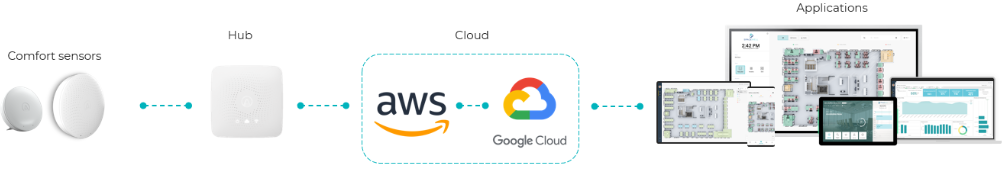
\includegraphics[scale=0.6]{figs/sb_airthingsNetwork.png}
    \caption{Reteaua Airthings}
    \label{fig:sb_airthingsNetwork}
\end{figure}

Modulul senzor are rolul de a achizitiona metrici de calitate a aerului si de a le transmite catre modulul Hub. Acesta functioneaza pe baterii si are o durata de 
viata de pana la 15 luni. Protocolul de comunicatie utilizat in reteaua interna compusa din senzori si gateway se numeste SmartLink si este un protocol proprietar 
dezvoltat de compania Airthings. Banda de frecventa in care senzorii comunica cu gatewayul este 868 MHz pentru Europa si 915 MHz pentru Statele Unite. Utilizarea 
acestei benzi de frecventa ofera o raza de acoperire a comunicatiei mai mare decat banda 2.4 GHz, mai ales in spatii inchise care contin multe obstacole.

Modulul Hub reprezinta gatewayul sistemului. Acesta are rolul de interfata intre senzori si internet, centralizand datele receptionate de la senzori si tranferandule 
mai departe in cloud. Conexiunea la internet se poate realiza prin cablu ethernet sau printr-o cartela SIM preinstalata de producator. Numarul maxim de senzori care 
pot fi conectati la modulul Hub este 10.

Modulul Cloud are rolul de a salva datele intr-o baza de date si de a oferi date istorice si date in timp real modulului Aplications.

Modulul Aplications ofera o interfata web sau pe telefonul mobil care afiseaza utilizatorului datele colectate de la senzori intr-un mod intuitiv.

Senzorii au capacitatea de a comunica si prin standarul Bluetooth direct cu aplicatia de pe telefonul mobil. In cazul acesta datele colectate de senzori sunt 
mentinute in memoria acestuia si transferate catre aplicatie atunci cand exista conexiune Bluetooth. Aplicatia are capacitatea de a monitoriza mai multi senzori 
in acelasi timp daca exista conexiune.

Airthings ofera mai multe tipuri de senzori care se deosebesc prin metricile de calitate a aerului colectate. Cel mai complex dintre acestea este Airthings Wave 
Plus care colecteaza urmatoarele metrici:
\begin{itemize}
	\item Gazul radioactiv Radon.
	\item Dioxid de Carbon (CO2).
	\item Concentratia Compusilor Organici Volatili Totala (TVOC)
	\item Umiditate.
	\item Temperatura.
	\item Presiunea Aerului.
\end{itemize}

\subsection{Avantaje}\label{subsec:airthings_avantaje}
\begin{itemize}
	\item Colectarea metricii radon.
	\item Functionarea pe baterii pana la 15 luni.
\end{itemize}

\subsection{Dezavantaje}\label{subsec:airthings_dezavantaje}
\begin{itemize}
	\item Numarul maxim de 10 senzori suportati de gateway este mic in cazul cladiririlor de birouri.
	\item Fara achizitionarea unui gateway, datele istorice care pot fi accesate sunt pe o perioada foarte scurta, limitata de memoria interna a senzorilor.
\end{itemize}

\section{Solutia Awair}\label{sec:awair}
\subsection{Descriere}\label{subsec:awair_descriere}
Solutia oferita de compania Awair este asemanatoare cu cea oferita de compania Airthings. Aceasta se concentreaza pe spatii inchise si include senzori de calitate 
a aerului, un gateway in anumite configuratii de retea, un server in cloud si aplicatie web sau pe telefon pentru gestiunea datelor. Ofera doua tipuri de senzori, 
unul pentru locuinte si unul pentru cladiri mari, cum ar fi scoli sau cladiri de birouri.

Solutia oferita de Awair pentru locuinte este senzorul Awair Element. Acesta este un senzor de sine statator capabil de crearea unei conexiuni prin protocolul 
Bluetooth sau prin protocolul Wi-Fi. Acesta este destinat pentru utilizarea impreuna cu un router uzual. Conexiunea Bluetooth este utilizata la instalarea senzorului 
unde, prin aplicatia pentru telefon Awair Home se realizeaza conexiunea Bluetooth si se transmit catre senzor informatii despre routerul la care acesta urmeaza sa 
se conecteze. La finalul procesului de instalare senzorul opreste conexiunea Bluetooth cu telefonul si se conecteaza la routerul despre care a primit informatii 
prin protocolul Wi-Fi. Din acest moment senzorul transmite periodic date catre serverul cloud. Aceasta solutie este foarte asemanatoare cu lucrarea de fata, cu 
exceptia capabilitatii de conectare prin Bluetooth pentru procesul de instalare.

Pentru spatii inchise mari Awair ofera o alta solutie care contine unul sau mai multi senzori numiti Awair Omni si un gateway numit Await Net. Senzorul Awair 
Omni este capabil de realizarea a trei tipuri de conexiuni:
\begin{itemize}
	\item Bluetooth - pentru procesul de instalare al senzorului.
	\item Wi-Fi - pentru utilizarea senzorului Awair Omni in acelasi mod in care este utilizat Awair Element.
	\item LoRa - pentru comunicatia dintre senzori si gateway.
\end{itemize}
Gatewayul Await Net poate fi conectat la internet utilizand un cablu ethernet sau o cartela SIM. Acesta comunica cu senzorii utilizand un protocol de comunicatie 
proprietar la baza caruia, in nivelul fizic al stivei de comunicatie, se afla tehnica LoRa. Banda de frecventa in care acesta comunica este 868 MHz pentru Europa 
si 915 MHz pentru Statele Unite. Senzorii au capabilitatea de repetor, ceea ce ofera posibilitatea crearii unei retele mesh. Distanta la care senzorii comunica 
in linie dreapta fara obstacole este de aproape un kilometru, iar prin capacitatea crearii unei retele mesh aceasta poate fi extinsa. In reteaua mesh fiecare 
senzor are un nod principal prin care comunica si o lista de cai secundare utilizate in cazul deteriorarii comunicatiei sau a caderii conexiunii cu nodul principal.

Senzorii sunt alimentati de la o sursa de 5V printr-un cablu USB type-C si achizitioneaza urmatoarele metrici de calitate a aerului:
\begin{itemize}
	\item Particulele in suspensie PM2.5 si PM10.
	\item Dioxid de Carbon (CO2).
	\item Concentratia Compusilor Organici Volatili Totala (TVOC).
	\item Umiditate.
	\item Temperatura.
	\item Lumina ambientala.
	\item Zgomotul ambiental.
\end{itemize}

Un al treilea tip de senzor oferit de awair se numeste Glow C, iar scopul acestuia este de integrare cu sistemele existente in locuinte sau in cladirile de birouri 
care nu suporta o conexiune Wi-Fi. Acest senzor este o extensie de stecher cu o priza care are capabilitatea de conectare Wi-Fi. In priza oferita de senzor poate fi 
conectat un sistem care nu suporta conexiune Wi-Fi, iar acesta va fi controlat de catre senzor prin pornirea si oprirea alimentarii bazat pe datele de calitate a 
aerului colectate de acesta. Exemple de astfel de sisteme sunt: un ventilator, un calorifer electric etc. De asemenea, acesta ofera o sursa de lumina LED care isi 
schima culoarea in functie de calitatea aerului detectat: Verde insemnand o calitatea a aerului buna, portocaliu insemnand o calitate a aerului acceptabila si rosu 
insemnand o calitate a aerului slaba.

Majoritatea senzorilor oferiti de Awair pot fi integrati cu asistentii virtuali Alexa, Google Home sau IFTTT.

\subsection{Avantaje}\label{subsec:awair_avantaje}
\begin{itemize}
	\item Capacitatea de acoperire a unei arii foarte mari datorata utilizarii protocolului LoRa si al capacitatii de creeare a unei retele mesh.
	\item Integrarea cu sisteme care nu suporta conexiune fara fir.
\end{itemize}

\section{Solutia Air Quality Egg}\label{sec:airqualityegg}
\subsection{Descriere}\label{subsec:airqualityegg_descriere}
Solutia oferita de compania Air Quality Egg este o platforma de dezvoltare destinata persoanelor pasionate de domeniul calitatii aerului. Datele colectate de catre 
senzorii din intreaga lume sunt disponibile intr-o platforma web oricarei persoane interesate in analiza acestora.

Senzorul, numit The Egg, este format dintr-o platforma hardware ale carei detalii sunt publice si utilizeaza un software care, la randul lui, este public. Aceste 
informatii sunt publice in scopul dezvoltarii rapide, orice persoana poate oferi solutii la probleme curente sau poate aduce imbunatatiri sistemului. Toti senzorii 
Egg colecteaza urmatoarele metrici de calitate a aerului: temperatura, umiditate si presiune. Pe langa acestea, la comandarea unui senzor nou este oferita o 
lista cu metrici suplimentare de calitate a aerului din care pot fi selectate cele dorite de cumparator. Acest lucru inseamna ca Air Quality Egg incepe productia 
unui senzor doar dupa plasarea unei comenzi, ceea ce face ca durata de receptie a senzorului sa fie mai lunga, aproximativ 4 saptamani.

Figura \ref{fig:sb_airqualityeggmap} prezinta senzorii Egg din intreaga lume. Afiseaza numarul de senzori instalati in fiecare locatie si un cod de culoare care 
prezinta calitatea aerului raportata de senzorii din locatia respectiva de la foarte buna la foarte slaba. Senzorii Egg care apar gri si transparenti reprezinta 
senzori care au pierdut conexiunea.
\begin{figure}[H]
    \centering
    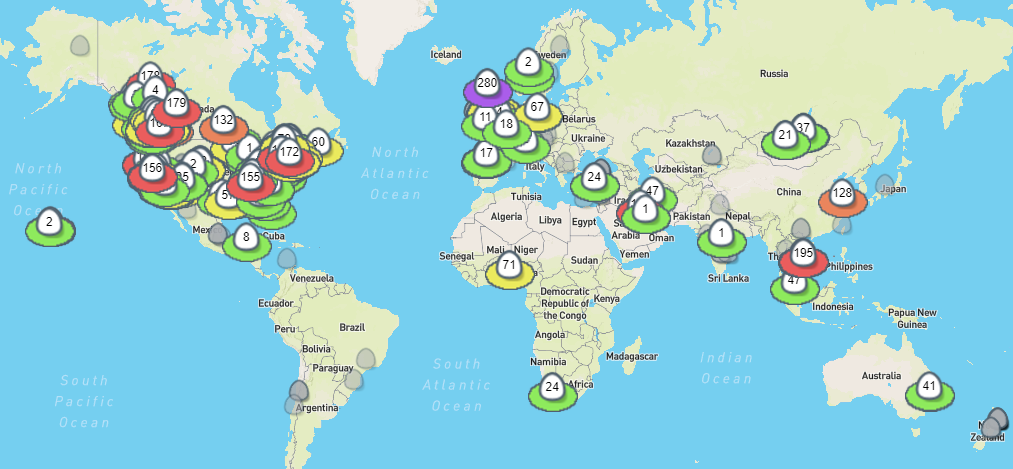
\includegraphics[scale=0.58]{figs/sb_airqualityeggmap.png}
    \caption{Harta senzorilor Egg}
    \label{fig:sb_airqualityeggmap}
\end{figure}

Aplicatiile web si pentru telefon smart ofera posibilitatea de vizualizare a datelor in timp real si a datelor istorice sub forma grafica sau ca valori de sine 
statatoare. De asemenea, aceste date sunt acompaniate de un cod de culori. Fiecare culoare corespunde unui interval de valori al indicelui de calitate al 
aerului (AQI):
\begin{itemize}
	\item Intervalul [0, 50] semnifica o calitate a aerului buna si este reprezentata prin culoarea verde.
	\item Intervalul [51, 100] semnifica o calitate a aerului moderata si este reprezentata prin culoarea galbena.
	\item Intervalul [101, 150] semnifica o calitate a aerului nesanatoasa pentru persoane sensibile si este reprezentata prin culoarea portocaliu.
	\item Intervalul [151, 200] semnifica o calitate a aerului nesanatoasa si este reprezentata prin culoarea rosie.
	\item Intervalul [201, 300] semnifica o calitate a aerului foarte nesanatoasa si este reprezentata prin culoarea mov.
	\item Intervalul [301, 500] semnifica o calitate a aerului riscanta si este reprezentata prin culoarea maro.
\end{itemize}

Procesul de instalare si configurare al unui senzor Egg este realizat prin conectarea acestuia la un calculator si utilizarea unei aplicatii oferita de Air 
Quality Egg. Cu ajutorul acestei aplicatii sunt transmise senzorului informatiile necesare pentru ca acesta sa se conecteze la un router (SSID, parola). De 
asemenea, aplicatia aceasta poate fi utilizata si pentru colectarea metricilor de calitate a aerului prin portul serial in cazul in care nu se doreste conectarea 
acestuia la un router. Senzorul este alimentat de la o sursa de 5V prin cablu USB.

Dupa procesul de instalare senzorul va incepe sa transmita datele colectate in serverul cloud si vor fi disponibile in aplicatiile web si de pe telefonul smart.

Platforma hardware a senzorului utilizeaza controlerul de retea CC3000 de la Texax Instruments pentru realizarea conexiunii Wi-Fi si poate contine senzori pentru 
colectarea metricilor de calitate a aerului prezentate mai jos. Un singur senzor nu poate contine toate aceste metrici, toti senzorii colecteaza metricile pentru 
temperatura, umiditate si presiune barometrica, iar in functie de urmatoarele metrici alease se poate ca altele sa nu mai poate fi integrate in senzor. De exemplu, 
daca se alege colectarea metricilor aditionale CO2, SO2 si NO2, nu mai este permisa adaugarea in senzor si a metricilor O3, H2S sau CO.
\begin{itemize}
	\item Particulele in suspensie OM1.0, PM2.5 si PM10.
	\item Dioxid de Carbon (CO2).
	\item Concentratia Compusilor Organici Volatili Totala (TVOC).
	\item Umiditate.
	\item Temperatura.
	\item Dioxid de sulf (SO2). 
	\item Ozon (O3).
	\item Dioxid de Nitrogen (NO2).
	\item Monoxid de carbon (CO).
	\item Sulfat de Hidrogen (H2S).
\end{itemize}

\subsection{Avantaje}\label{subsec:airqualityegg_avantaje}
\begin{itemize}
	\item Platforma hardware care poate fi personalizata.
	\item Vizualizarea si capabilitatea de analizare a datelor raportate de senzorii Egg din intreaga lume.
	\item Posibilitatea de inlocuire a componentelor senzorului.
\end{itemize}

\section{Solutia PurpleAir}\label{sec:sb_purpleair}
\subsection{Descriere}\label{subsec:sb_purpleair_descriere}
Solutia oferita de compania PurpleAir se concentreaza pe impartasirea datelor colectate cu intreaga lume prin platforma oferita de acestia. Ofera patru variante 
de senzori de calitate a aerului care au capabilitatea de conectare la un server cloud. Trei dintre aceesti senzori sunt destinati pentru spatii inchise, spatii 
deschise sau domeniul industrial, iar al patrulea este destinat doar pentru spatii inchise.

Senzorii destinati pentru spatii deschise sau domeniul industrial sunt incapsulati intr-o cutie rezistenta la conditiile meteo din spatiile deschise si la 
conditiile extreme din domeniul industrial cum ar fi, temperaturi extreme sau umiditate crescuta. Acestia au capabilitatea de functionare fara conexiune Wi-Fi 
utilizand un card de memorie de maxim 64 GB de pe care datele pot fi extrase prin portul Micro USB. Tot prin portul Micro USB se realizeaza si alimentarea 
acestora cu 5V.

Pentru instalarea senzorului in cazul in care se doreste adaugarea acestuia intr-o retea Wi-Fi este necesara utilizarea unui computer sau a unui telefon smart 
cu capabilitatea de conectare la o retea Wi-Fi. La prima utilizare sau dupa o resetare a senzorului acesta intra in modul AP in care se comporta ca un router cu 
capabilitatea de conectare a unui singur device. Senzorul va aparea in lista de retele Wi-Fi cu denumirea "PurpleAir\_[numele senzorului]". Informatiile despre 
reteaua locala la care se doreste conectarea senzorului, SSID, parola etc, sunt transmise prin conectarea la reteaua creata de senzor si accesara unei pagini 
web de configurare. La finalul procesului de instalare, senzorul va opri reteaua locala creata, se va conecta la routerul despre care a primit informatii 
si va incepe sa transmita date periodic catre serverul din cloud.

Figura \ref{fig:sb_purpleairmap} prezinta harta snezorilor pusa la dispozitie de PurpleAir pentru vizualizarea calitatii aerului din intreaga lume. Pentru 
ca un senzor sa apara pe aceasta harta si pentru ca datele colectate de acesta sa poata fi accesate de orice persoana, senzorul trebuie inregistrat de catre 
utilizator in platforma PurpleAir. 
\begin{figure}[H]
    \centering
    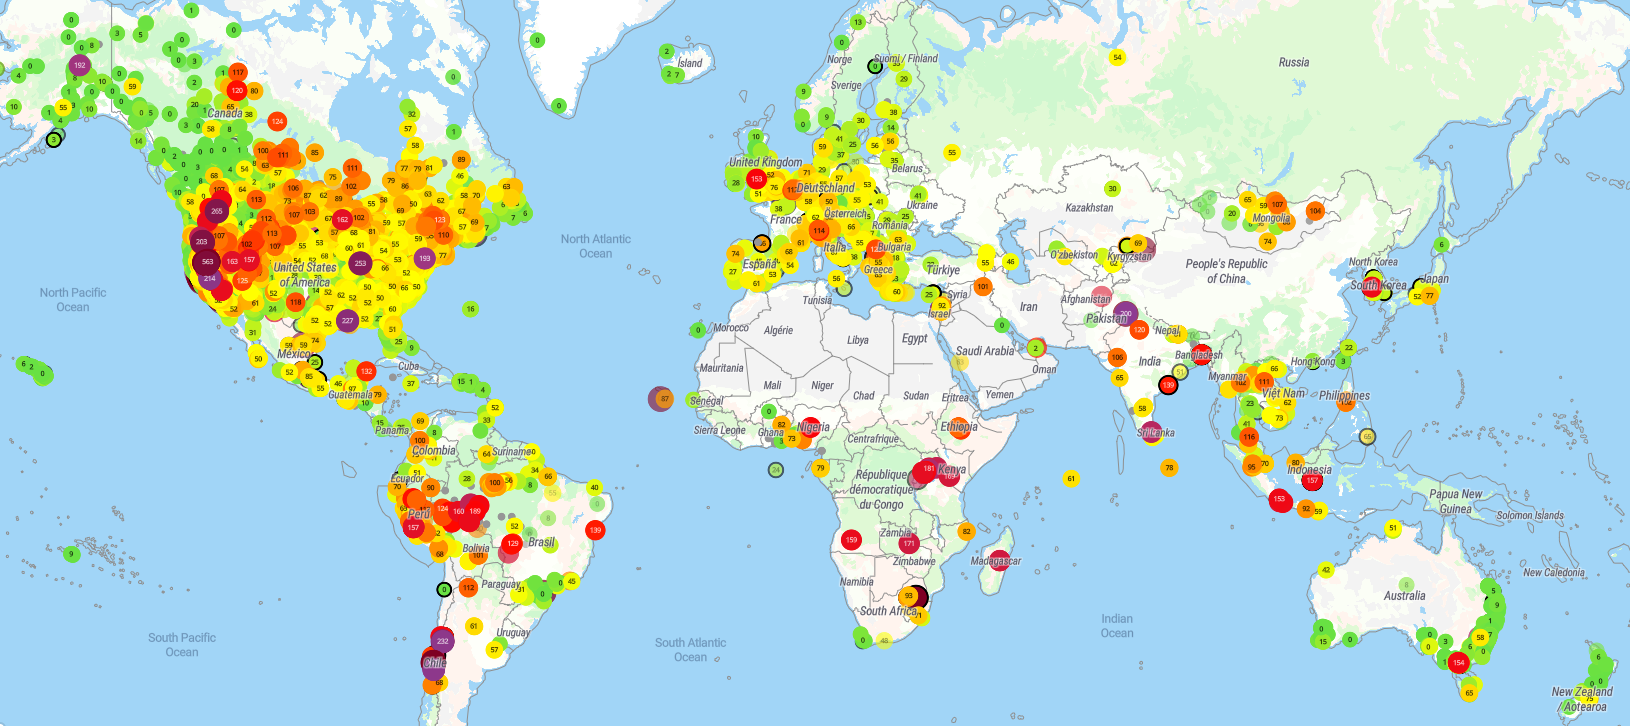
\includegraphics[scale=0.35]{figs/sb_purpleairmap.png}
    \caption{Harta senzorilor PurpleAir}
    \label{fig:sb_purpleairmap}
\end{figure}

In cazul conectarii senzorului la o retea locala fara access la internet, datele colectate de acesta pot fi accesate prin introducerea manuala a unei adrese 
URL in browserul web. Primul pas in aceasta procedura este identificarea IP-ului pe care senzorul la primit la conecarea in reteaua locala. Pentru acest lucru 
este necesara accesarea paginii de configurare a routerului si identificarea manuala, dintr-o lista de IP-uri, a IP-ului specific senzorului. Adresa URL 
introdusa in browserul web reprezinta o cerere HTTP de tip GET al carei raspuns este afisat in pagina web in format JSON.

Metricile de calitate a aerului colectate de senzori sunt:
\begin{itemize}
	\item Particulele in suspensie PM1.0, PM2.5, PM10.
	\item Presiune.
	\item Umiditate.
	\item Temperatura.
	\item Gaz.
\end{itemize}
Pentru colectarea metricilor OM1.0, PM2.5 si PM10 este utilizat senzorul PMS-x0003 de la Plantowner. Fiecare senzor detinut de AirPurple contine doua 
unitati PMS-x0003 pentru redundanta, iar pentru colectarea metricilor de presiune, temperatura, umiditate si gaz este utilizat senzorul BME688 de la BOSH. Pentru 
conexiunea Wi-Fi, snezorii utilizeaza controlerul de retea ESP-WROOM-02D de la Espressif Systems. Toti senzorii utilizati in acest paragraf sunt destinati pentru 
utilizarea in domeniul industrial avand intervalul de temperatura de functionare [-40, +85] grade celsius.

\subsection{Avantaje}\label{subsec:sb_purpleair_avantaje}
\begin{itemize}
	\item Platforma software pentru vizualizarea senzorilor si a calitatii aerului din intreaga lume.
	\item Posibilitatea de inlocuire a componentelor senzorilor.
\end{itemize}
\subsection{Dezavantaje}\label{subsec:sb_purpleair_dezavantaje}
\begin{itemize}
	\item Senzorul utilizeaza protocolul HTTP pentru transmisia datelor catre server. Acesta reprezinta un dezavantaj deoarece protocolul HTTP este destinat 
	pentru transmisia paginilor web si nu este potrivit pentru formatul datelor transmise de senzor.
	\item Afisarea datelor catre utilizator in format JSON, un format greu de citit de catre utilizator.
\end{itemize}

{\color{blue}\noindent Acest capitol se va extinde pe de la 3 la 10 pagini.\\}

Documentarea bibliografică are ca obiectiv prezentarea stadiului actual al domeniului sau sub-domeniului în care se situează tema.
În redactarea acestui capitol (în general a întregului document) se va ține cont de cunoștințele acumulate la disciplinele dedicate din semestrul 2, anul 4
(Metodologia Întocmirii Proiectelor, etc.), precum și la celelalte discipline relevante temei abordate.


Referințele se scriu în secțiunea Bibliografie.

Formatul referințelor trebuie să fie de tipul IEEE sau asemănător.

Introducerea și formatarea referințelor în bibliografie, respectiv citarea în text, se pot face manual sau folosind instrumentele de lucru menționate în ultimele 
paragrafe din acest capitol.

Recomandăm gestiunea referințelor folosind \href{https://www.jabref.org/}{JabRef} care se poate descărca de la \url{https://www.jabref.org/#download}

Forma referințelor bibliografice pe categorii de referințe o puteți găsi \href{https://libguides.nps.edu/citation/ieee-bibtex}{aici}.

Despre erori comune de formatare ale referințelor din bibliotecile online puteți citi \href{https://www.ece.ucdavis.edu/~jowens/biberrors.html}{aici}


In capitolul~\ref{ch:analysis} din~\cite{strunk}, care tratează valoarea honeypots, Spitzner prezintă avantajele și dezavantajele acestor sisteme.


În secțiunea \textit{Bibliografie} sunt exemple de referințe pentru articol la conferințe sau seminarii~\cite{BellucciLZ04}, articol în jurnal~\cite{AntoniouSBDB07},
sau cărți~\cite{russell1995artificial}.


Referințele spre aplicații sau resurse online (pagini de internet) trebuie sa includă cel puțin o denumire sugestivă pe lâ ngă link-ul propriu-zis~\cite{webpage},
plus alte informații dacă sunt disponibile (autori, an, etc.).
Referințele care prezintă doar link spre resursa online se vor plasa în subsolul paginii unde sunt referite.
Citarea referințelor în text este obligatorie, vezi exemplul de mai jos (în funcție de tema proiectului se poate varia modul de prezentare a metodei/aplicației).

%În articolul~\cite{AntoniouSBDB07} autorii prezintă un sistem pentru ...
În~\cite{AntoniouSBDB07} autorii prezintă un sistem pentru detecția obstacolelor în mișcare folosind stereo viziune și estimarea mișcării proprii.
Metoda se bazează pe ...{\it trecerea în revistă a algoritmilor, structurilor de date, funcționalitate, aspecte specifice temei proiectului etc}. Discuție {\it avantaje - dezavantaje}.


\textit{De exemplu:} În capitolul numit "Problem-solving" din lucrarea~\cite{russell1995artificial} se prezintă ...

